
\section{Programs for Graphical display\index{display} of calculated data}
\label{graphics}

If java is installed on the system, running McPhase will
 display\index{display} the calculated magnetisation
curve immediately during the simulation updating 
it in regular intervals\footnote{Depending on the Java setup on your computer, a conflict may occur between the McPhase 
Java programs and other Java programs, such as the Matlab GUI. If you find that no graphics
windows open, and have other Java programs running in the background, try to close all other Java programs.}
(this can be done for any other
curve  by using the
program: {\prg display\index{display} x-colnr y-colnr filename}). 
Also the text in output files can be monitored by the program:
{\prg displaytext\index{displaytext} filename}.
During the simulation
the results are stored in the directory {\prg ./results}, the output files can be viewed 
using the programs described in this section. 

\subsection{Programs {\prg display},{\prg displaybubbles\index{displaybubbles} },{\prg %%@
displaycontour\index{displaycontour}},{\prg displaytext\index{displaytext}} and {\prg show} - graphical %%@
display\index{display} of any xy data such as magnetisation etc.}
\label{display}

\begin{description} 
\item [display\index{display} 1 11 ./results/mcphas.fum] produces a graphical display\index{display} of the data %%@
file
mcphas.fum on screen. The display\index{display} contains an xy plot of column 1 versus column 11
({\prg java} has to be installed to use this program). 
More files may be displayed by commands such as

{\bf display\index{display} 1 2 data1.dat 3 5 data2.dat}.

Note that viewing of 
data which is generated by programs may be viewed online. The program updates the plot
every 500 milliseconds. In this way it is possible to watch online, how programs
calculate data. The output of display\index{display} may contain lines to tune the display\index{display} output, %%@
such as
\begin{verbatim}
	most general usage: 

 display [-options] xcol[excolerr] ycol[eycolerr][bcolbubble] file [xcol1[] ycol1[] file1 ...]


xcol,ycol ... column to be taken as x-, y- axis  in a lineplot
when using option -o file.jpg the application creates a jpg file on exiting
when using option -xmin 23.3 the application sets the minimum of the display xaxis to 23.3
similar are options -xmax -ymin -ymax ....
when using option -c file.jpg the application only creates a jpg file and exits immediatly
if optional errorcolumns are added then instead of lines symbols and errorbars are shown
if optional bubblecolumns are added then instead of lines bubbles with area corresponding to
bubblecolumn are shown (toggle bubblesize with 's' and 'b')
(toggle lines also with '-' key))
filename ..... filename of datafile
Data files may contain lines to tune the display output, such as
#! displaytitle=My new Graph
#! displayytext=intensity
#! displayxtext=meV 
\end{verbatim} 

\item [displaybubbles\index{displaybubbles}  5 6 8 ./results/mcdisp.qei] works similar as display, however
a third column is given and the radius of the symbols varied according to the data in 
this column.

\item [displaycontour\index{displaycontour} 5 6 8 ./results/mcdisp.dsigma.tot] produces a graphical
display\index{display} of a 3 dimensional dataset as a colour and/or contour plot. Here '5 6 8' 
denote the x,y and z column in file {\prg ./results/mcdisp.dsigma.tot}, which should
be plotted. Figure~\ref{ho2ti2o7diffuse} shows an sample output of this program. The axes labels may be changed
in Tree View $\rightarrow$ xaxis title, etc.

\item [displaytext\index{displaytext} ./results/mcphas.hkl] monitors the file mcphas.hkl in a text window
on screen.
\end{description} 

\subsection{Programs {\prg display\_density}\index{display\_density} 
- display of the charge- spin- moment- current- density of a single ion}\label{displaydensity}

The program {\prg display\_density}\index{display\_density} is used to display a surface of constant
charge density for an open shell ion, which is described by a single ion property file.
In addition, also, the spin-, orbital moment, total magnetic moment and orbital current
densities can be displayed. 


\begin{description} 
\item [ display\_density\index{display\_density}  c$|$s$|$o$|$m$|$j [-p i j k$|$-div] [-S$|$-L$|$-M] mcphas.sipf
 T Ha Hb Hc]
\end{description} 
\begin{verbatim}
                 c ... calculate chargedensity
                 s ... calculate spindensity
                 o ... calculate angular orbital momentum density
                 m ... calculate magnetic moment density
                 j ... calculate currentdensity
        optional p i j k ... calculate projection of spin/orbital/current/magnetic 
                             moment density along direction i j k, e.g. 0 0 1
        optional -div    ... calculate divergence of spin/orbital/current/magnetic 
                             moment density
        optional -S  ... show arrow indicating spin
        optional -L  ... show arrow indicating orbital angular momentum
        optional -M  ... show arrow indicating magnetic moment
                 - crystal field  parameters Blm should be read from a
                   standard mcphas single ion property file mcphas.sipf
                 - given is temperature T[K] and magnetic effective field H[T]
                options: if T<0 then no thermal boltzmann distribution is taken
                the statistical probability of each CF state has to be entered
                by hand.
     example:
               display_density c Pr3p.sipf 2 0 0 1
             ...calculates the charge density using crystal field from Pr3p.sipf
                at T=2K and H=(0,0,1) Tesla
\end{verbatim}

Note: if T$<$0, then no thermal Boltzmann distribution is taken - 
		the statistical probability of each CF state has to be 
		entered by hand.

For the calculation of the charge density the  formula are used as given in
appendix~\ref{chargedensityoperator}. 
Spin-, Moment- and Currentdensities
currently only available in combination with module {\prg ic1ion\index{ic1ion}}.
Formalism based on \cite{balcar75-1581,balcar89-1,rotter11-12005}.


Technical information: the program {\prg display\_density} is actually a script which
calls  {\prg densplt\index{densplt}} 
 (a program with the same arguments as {\prg display\_density}
which calculates the iso surfaces and stores
it in format for the java based graphic program {\prg javaview} and
also as a grid. The way in which this is done is controlled by 
the parameter file {\prg results/graphic\_parameters.set}
.... in  order to display the results graphically the following java
programs are called:
\begin{verbatim}
 javaview results/densplt.jvx
 displaycontour 2 3 4 results/densplti.grid
 displaycontour 1 3 4 results/denspltj.grid
 displaycontour 1 2 4 results/denspltk.grid
\end{verbatim}

Note on javaview: You can create also several plots (for instance for different temperatures) and store these
in a sequence such as densplt.1.jvx, densplt.2.jvx, ... animate
the view of 4 jvx files by typing: java javaview model=densplt.*.jvx Animation.LastKey=4 


\subsection{Programs {\prg display\_densities}\index{display\_densities}  - display of the superstructure
and excitations}\label{displaydensities}


The program {\prg display\_densities}\index{display\_densities} 
can be used simply to popout spin/exchange field configuration 
and also to display a 3d animation of spin/moment/densities, even including a movie of
excitations.

\begin{figure}[hb]%h=here, t=top, b=bottom, p=separate figure page
\begin{center}\leavevmode
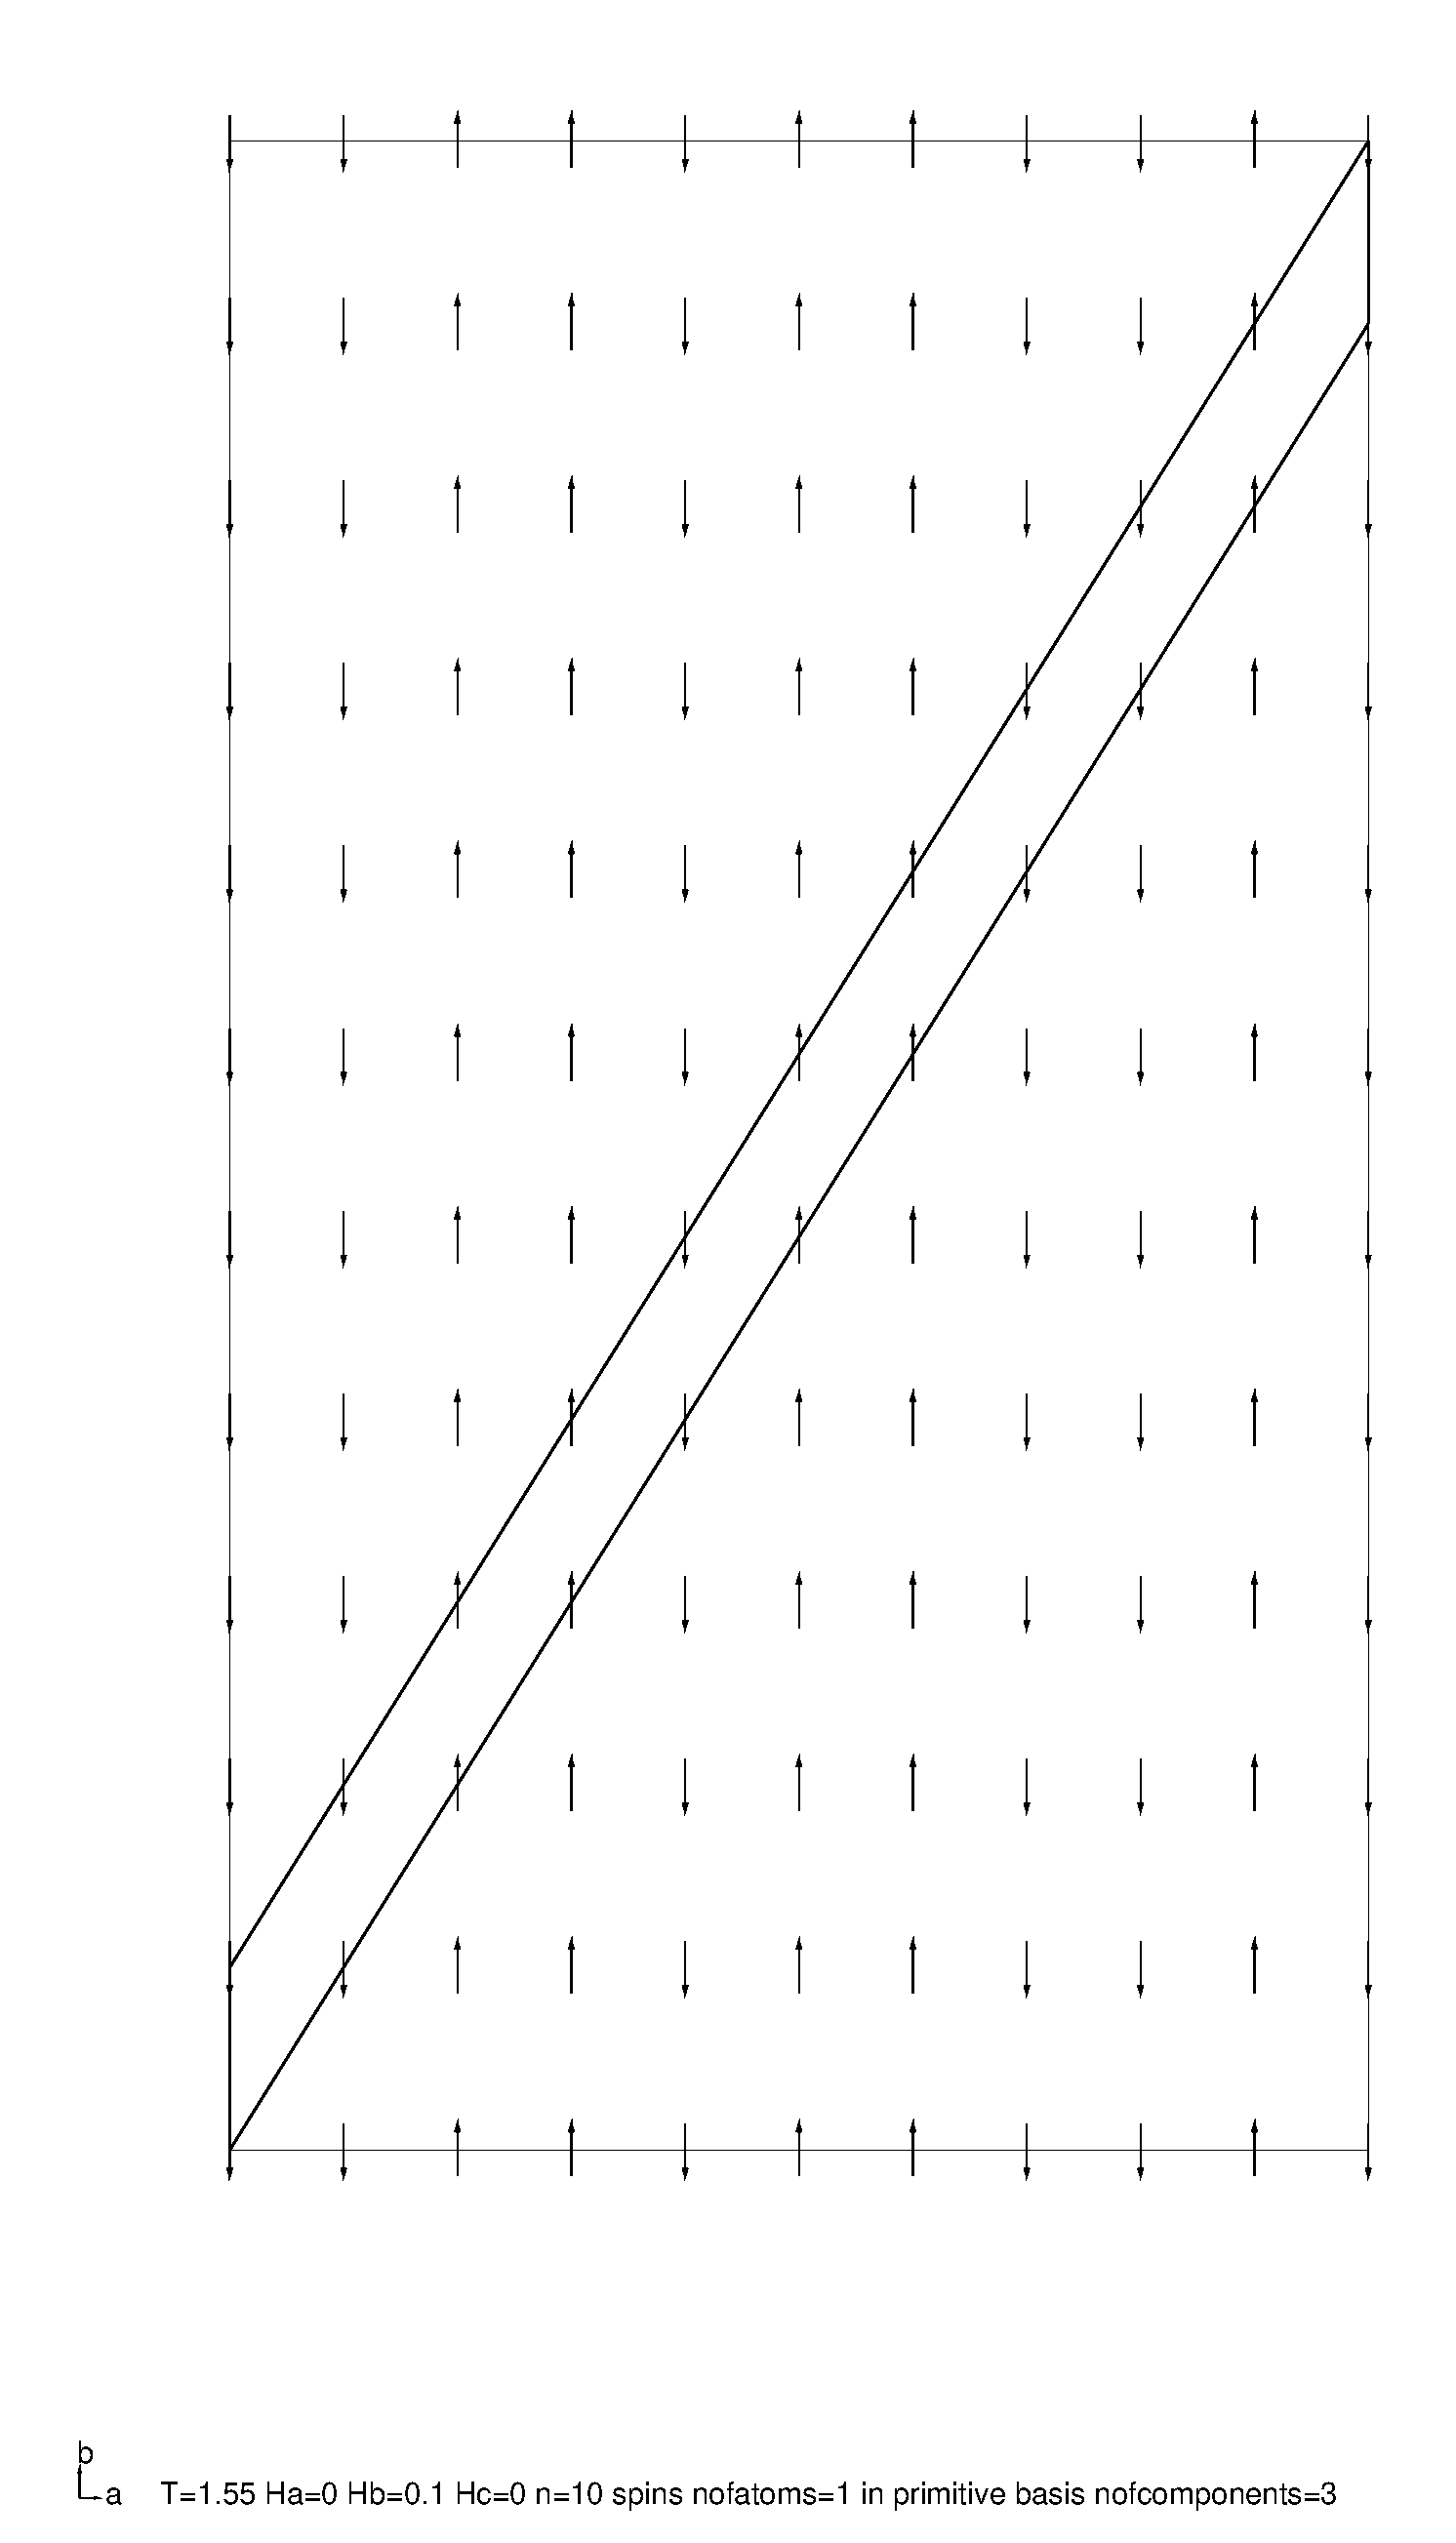
\includegraphics[angle=0, width=1.0\textwidth]{figsrc/ndcu2b/resultss/spinsab.eps}
\end{center}
\caption{Calculated Spin-Structure of NdCu$_2$ at $T=$~1.5~K and $H=0$.
[plot created by program {\prg display\_densities}\index{display\_densities}]}
\label{spingraphic}
\end{figure}





\begin{description} 
\item[ display\_densities -f mcphas.sps T Ha Hb Hc]
 if used with -f filename this file has to be a mcphas.mf or mcphas.sps file,
the spin configuration
   at given temperature T[K] and magnetic effective field H[T]
    is read and extracted from this file and printed on screen (stdout), nothing
 else is done
\item[display\_densities [-c$|$-s$|$-o$|$-m$|$-j] [-p i j k$|$-div] [-S$|$-L$|$-M] [-P] T Ha Hb Hc [h k l E]]
 if used without a filename, the information is read from results/mcphas.* res
ults/mcdisp.*
   output files and 3d graphical animations are created.
\end{description} 
\begin{verbatim}
   options are:
         -c ... calculate chargedensity
         -s ... calculate spindensity
         -o ... calculate angular orbital momentum density
         -m ... calculate magnetic moment density
         -j ... calculate currentdensity
         -p i j k ... calculate projection of spin/orbital/current/magnetic moment density
                  along direction i j k, e.g. 0 0 1
         -div    ... calculate divergence of spin/orbital/current/magnetic moment density
         -S  ... show arrow indicating spin
         -L  ... show arrow indicating orbital angular momentum
         -M  ... show arrow indicating magnetic moment
         -P  ... calculate phononic displacement
         note, that in order to animate changes in the above quantities, the corresponding
         switch has to be enabled in the mcdisp calculation (mcdisp.par) and the single ion
         modules have to be capable of calculating the corresponding observables.

     example:
        display_densities -c 2 0 0 1
        ...calculates the charge density at T=2K and H=(0,0,1) Tesla
\end{verbatim}

\begin{figure}[hb]%h=here, t=top, b=bottom, p=separate figure page
\begin{center}\leavevmode
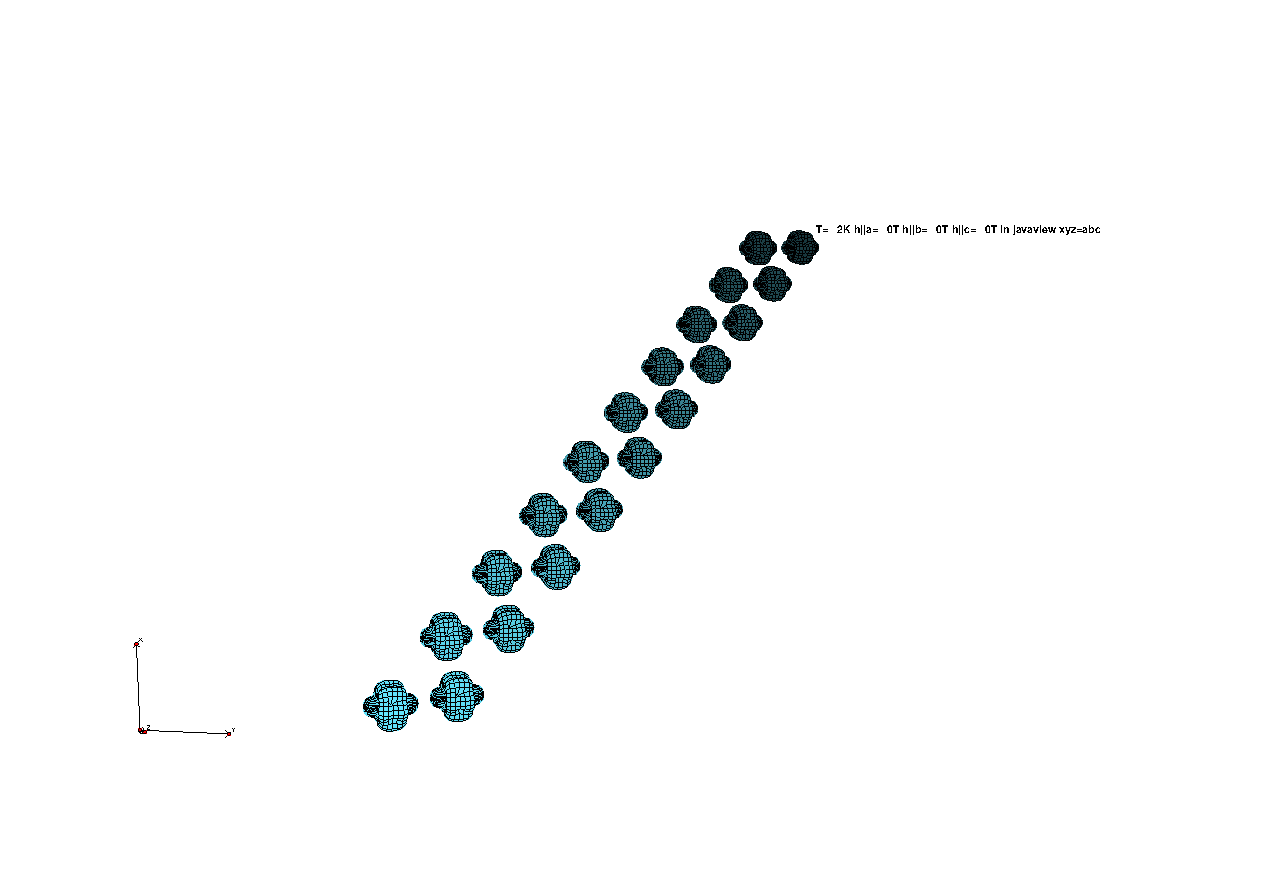
\includegraphics[angle=0, width=0.7\textwidth]{figsrc/ndcu2b/resultss/chargesab.eps}
\end{center}
\caption{Calculated 4f Charge-Structure of NdCu$_2$ at $T=$~1.5~K and $H=0$.
[plot created by program {\prg display\_densities}\index{display\_densities}]}
\label{chargegraphic}
\end{figure}

The program can be used to calculate (partial) chargedensity for the unfilled shells
 of magnetic ions in  a magnetic unit cell, which has been calculated by {\prg mcphas} and
 stored in {\prg mcphas.mf} for a specific temperature and magnetic field.
   For the calculation of the charge density the  formula are used as given in
appendix~\ref{chargedensityoperator}. 
In order to do so {\prg display\_densities}\index{display\_densities}  requires input files and the result of a
full {\prg mcphas} simulation.
Alternatively, {\prg display\_densities}\index{display\_densities}
can  calculate the spindensity, the orbital magnetic moment density, the total magnetic
moment density (in Trammel gauge) and the (orbital) electric current density.

 The program outputs a magnetic structure (and magnetic excitation)
  graphic/movie in the output files of different format:
  results/spins*.eps (postscript), results/spins*.fst (fp\_studio),
  results/spins.out (ascii) and results/spins*.jvx (javaview).

Output files:
\begin{enumerate}
  \item encapsulated postscript ps-file {\prg results/spins*.eps}
                  of a spin/orbital/totalmagnetic moment configuration, 
  \item the files {\prg results/spins.fst} and {\prg results/spins\_prim.fst} are created, 
                which can be read by the fullprof program {\prg fp\_studio}
                for on screen display\index{display} of a spin/orbital/totalmagnetic moment configuration,
  \item the configuration of expectation values $\langle\mbf I\rangle$ (or whatever is stored in the file addressed by the option -f)
                 is printed to stdout - therefore this program can be used with option {\prg -f results/mcphas.mf} 
			       to generate an input file
			       for program {\prg  McDisp} (example: {\prg spins -f results/mcphas.mf 1 1 0 0  $>$ mcdisp.mf})  
  \item the text file {\prg results/spins.out} is created, which is useful to produce input files for
              the diffraction program {\prg mcdiff\index{mcdiff}} (done in the script {\prg setup\_mcdiff\_in})
  \item the graphics files {\prg results/spins.jvx} and {\prg results/spins\_prim.jvx}, which can be displayed
         by the program {\prg javaview}, e.g. by the command {\prg java javaview spin\_prim.jvx}.
  \item if {\prg spins} is used with arguments {\prg h k l E(meV)}, it takes the eigenvectors of magnetic 
excitations
        from files {\prg results/mcdisp.q*}  created by {\prg mcdisp}) and produces a graphical
        animation of the spin osciallation which is associated with this magnetic mode. The output is a series
        of files {\prg results/spins.*.jvx} and {\prg results/spins\_prim.*.jvx} which can be viewed by program
        {\prg javaview}, e.g. by the command {\prg java javaview "model=results/spins\_prim.*.jvx" 
        Animation.LastKey=16 background="255 255 255"}.  {\prg javaview} is also able to produce a sequence
		of gif files (press c in the animation window), which can then be processed by an animation editor
		to generate an animation, which can be inserted in presentations. For example, you can use
 {\prg  Imagemagick} graphics package (has to be installed separately!)
        to create an animation. The following command will issue a proper gif animation, which you can include in 
           power point        
        presentations etc.: {\prg convert -delay 1 -size 100x100 -loop 1 geomAnim.*.gif output.gif}.
 \end{enumerate}

                          Note, in case of non-orthogonal axes the convention 
                           for applied field $Ha, Hb,Hc$ 
                            is $Hb||\vec b$, $Hc||(\vec a \times \vec b)$ and $Ha$ perpendicular to $Hb$ and $Hc$.


  The graphics output format can be fine tuned in {\prg results/graphic\_parameters.set} 
  by  {\prg spins\_scale\_moment},
{\prg show\_abc\_unitcell, show\_primitive\_crystal\_unitcell, show\_magnetic\_unitcell, show\_atoms, 
scale\_view\_1,
scale\_view\_2, scale\_view\_3},  
{\prg spins\_wave\_amplitude, spins\_show\_ellipses, spins\_show\_direction\_of\_static\_moment}.
{\prg show\_abc\_unitcell, show\_primitive\_crystal\_unitcell, show\_magnetic\_unitcell, show\_atoms, %%@
 show\_density}...

Technical information: the program {\prg display\_densities}\index{display\_densities} 
is actually a script which
calls  {\prg spins\index{spins}} 
 (a program with the same arguments as {\prg display\_densities}
which calculates the iso surfaces and stores
it in format for the java based graphic program {\prg javaview} and
also as a grid. The way in which this is done is controlled by 
the parameter file {\prg results/graphic\_parameters.set}
.... in  order to display the results graphically the following java
programs are called:
\begin{verbatim}
  java javaview results/spins.jvx
  java javaview "model=results/spins.*.jvx" Animation.LastKey=16 background="255 255 255"
\end{verbatim}







\subsection{Program {\prg hkl\index{hkl}}, {\prg hkl2d\index{hkl2d}} and {\prg mcdiff\index{mcdiff}} - graphical %%@
display\index{display} of magnetic diffraction intensity}
\begin{description} 
\item [{{\prg hkl\index{hkl}} [options] [file]} ]                   produces neutron intensity graphic
 and postscript-file {\prg hkl.ps}. {\prg perl} and
{\prg pgplot} must be installed in order to use this program.
 Options are -n (plot reflex number n)
-h (help). If no file is given the program uses file {\prg mcphas.hkl}.
\item [{{\prg hkl2d\index{hkl2d}} [options] [file]} ]   same as {\prg hkl\index{hkl}} but two-dimensional colour %%@
plot of intensity.
\end{description} 
the following example (fig.~\ref{neutintgraphic}) shows the temperature dependence of the neutron intensity
on the different harmonics of NdCu$_2$.

\begin{figure}[htb]%h=here, t=top, b=bottom, p=separate figure page
\begin{center}\leavevmode
\includegraphics[angle=-90, width=0.8\textwidth]{figsrc/ndcu2b/resultss/hkl.ps}
\end{center}
\caption{NdCu$_2$: calculated temperature dependence of magnetic amplitudes of the
main propagation vector and higher harmonics (at zero magnetic field).}
\label{neutintgraphic}
\end{figure}

In addition to the display\index{display} of the temperature dependence there is the
possibility to generate a powder diffraction pattern by the 
program mcdiff~\index{mcdiff}. The 
recommended procedure is to use 

\begin{description}
\item[{\prg setup\_mcdiff\_in\index{setup\_mcdiff\_in}} T Ha Hb Hc:] to generate a file {\prg mcdiff.in} which
contains the spin configuration, lattice etc. information at a
desired temperature. Edit this output file and at the beginning
of the file insert some additional information as described in section~\ref{mcdiff}.

Continue by using  the modules
\item[{\prg mcdiff\index{mcdiff}}:] as described in detail in section~\ref{mcdiff} to
generate a list of reflections with the corresponding neutron powder
intensities (file {\prg mcdiff\index{mcdiff}.out}). In order to create a powder pattern 
a further step is required using the program
\item[{\prg convolute\index{convolute}}... mcdiff\index{mcdiff}.out [+options] resolution file:]
  is also described in section~\ref{addprog}. This program convolute\index{convolute}s the
reflection list with a specific resolution function.
\end{description}

\clearpage

\subsection{Program {\prg phased} - graphical display\index{display} of magnetic phase diagrams}
\begin{description}
\item [phased    [file]]       produces graphic of magnetic xy($HT$)-phase diagram [file]. Note that
{\prg perl} and {\prg pgplot} are needed in order to use this program. Thus it is more
convenient to use {\prg displaycontour}:
\item [substitute "p " "  " results/mcphas.xyt] to substitute the p in the file with spaces
\item [displaycontour 1 2 8 results/mcphas.xyt] to display the phase indices as coloured phase diagram.
\end{description}

Mind that the plot produced is based on the phase number given in {\prg mcphas.xyt}, which may be
different for the ''same'' magnetic structure as mentioned above
(section~\ref{outputfiles}, {\prg mcphas.phs}). It is recommended to check carefully, if
some magnetic structures are physically equal, although numbered with different phase numbers by
the program. If such a case is detected, the phase numbers in {\prg mcphas.xyt} should
be put to the same value in order to be able to identify the stability region in the plot.

\begin{figure}[hb]%h=here, t=top, b=bottom, p=separate figure page
\begin{center}\leavevmode
\includegraphics[angle=-90, width=0.5\textwidth]{figsrc/ndcu2b/resultss/phased.ps}
\end{center}
\caption{Calculated magnetic phase diagram of NdCu$_2$ for field parallel to the orthorhombic $b$-direction.}
\label{phasediagramgraphic}
\end{figure}
\clearpage


\subsection{Program {\prg felog} - display\index{display} logged free energy for different moment configurations %%@
at a temperature/field (linux with pgplot grphic library only)}

\begin{description} 
\item [felog]                  produces plot of logged q values in reciprocal
space vs free energy (colours). {\prg pgplot} and {\prg perl} are needed in order
to use this graphical tool.
(Trick: in order to get a quick overview of the
q-vector range covered by the mcphas\index{mcphas} simulation just type {\prg felog ./results/mcphas.qvc})
\end{description} 

\begin{figure}[hb]%h=here, t=top, b=bottom, p=separate figure page
\begin{center}\leavevmode
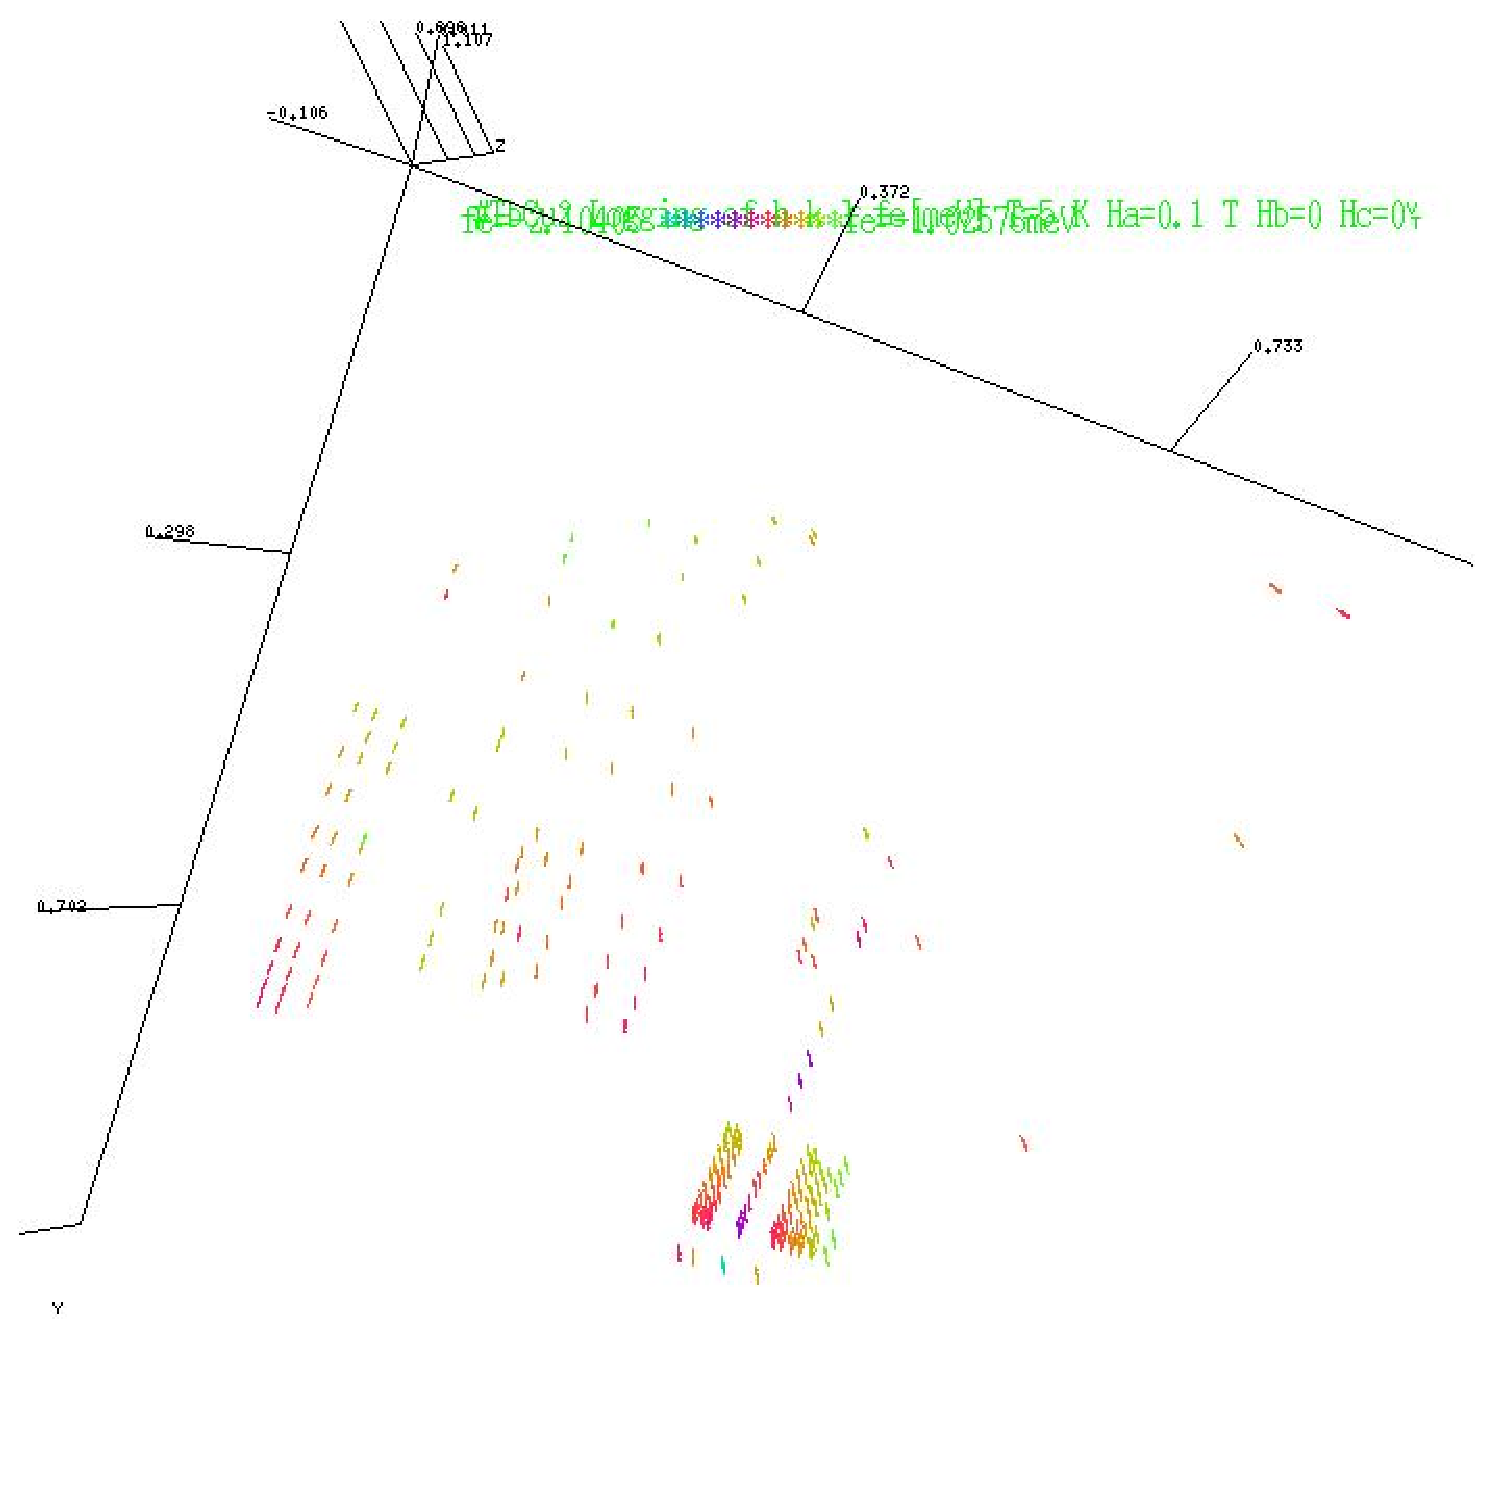
\includegraphics[angle=0, width=0.8\textwidth]{../demo/pictures/felog.eps}
\end{center}
\end{figure}

\vspace{1cm}
{\em Exercises:}
\begin{itemize}
\item Use the programs {\prg phased, hkl, hkl2d, spins, javaview} to generate
graphical output of the simulation results in directory 
{\prg examples/ndcu2b\_new/results}.
\end{itemize}


